\documentclass[arial,11pt]{article}
%\documentclass[11pt]{nih}
\usepackage{amssymb}
%\usepackage{graphicx}
%\usepackage{longtable}
\usepackage{epsfig}
\usepackage{overcite}

\renewcommand{\rmdefault}{phv} % Arial
\renewcommand{\sfdefault}{phv} % Arial
\pagestyle{empty}

%\usepackage{times}
\usepackage{geometry}
%\geometry{tmargin=1in,bmargin=1.0in,lmargin=1in,rmargin=1in}
\geometry{tmargin=0.95in,bmargin=0.95in,lmargin=0.95in,rmargin=0.95in}
%\linespread{0.95} \interfootnotelinepenalty=10000

%%%%% editing helpers
\newcommand{\NeedRevision}[1]{\textcolor{red}{#1}}

\begin{document}

\section{Specific aims}
%\subsection{}
%\subsection{}
\subsection{\textbf{Aim 3: Universal tools for identification of linked peptides}}

Most existing database search tools are designed for and trained on MS/MS data from linear peptides.  However in many biological applications, the identification of linked peptides is crucial.  These present a challenge for current computational tools because: 1) linked peptides have substantially different fragmentation patterns as compared to linear peptides; 2) fragment ions from more than one peptide are present in the same MS/MS spectrum and 3) there are usually too few examples of annotated spectra from linked peptides in the literature to learn their fragmentation patterns.  To address these challenges we will generate large MS/MS training data from linked peptides using combinatorial peptide synthesis. From this training data, we will develop an algorithm UniLink that can automatically learn a probabilistic model specific for linked peptides and use this to identify MS/MS spectra from \emph{any} linked peptides accurately and efficiently.

%*******************************************
\section{Significance}
%*******************************************
Linked peptides can be defined as two (or more) covalently linked peptides. These can arise naturally from biological samples \-- for example, posttranslational modifications (PTMs) such as Ubiquitination, PUPylation and Small Ubiquitin-like Modification (SUMOylation)~\cite{pickart2001mechanisms,hochstrasser2009origin,geiss2007concepts}, which involves small modifier proteins of around 100 amino acids that reversibly attach to substrate proteins to modify their function. These PTMs are involved in many cellular pathways such as cell death, cellular trafficking, cell cycle, DNA repair and replication~\cite{meulmeester2008cell}. In particular, SUMOylation has been implicated in neural degenerative diseases such as Alzheimer's disease  and Huntington disease\cite{zhang2008sumoylation,steffan2004sumodis}. Upon enzymatic digestion of the modified substrate proteins, substrate peptides that contain the PTM conjugation site will be covalently linked to a C-terminal remnant or ``tag'' of the modifier protein, resulting in a ``y-shaped'' linked peptide (Figure~\ref{linkedmodel}). Unbiased detection of linked peptides provide direct evidence that a protein is a substrate for modification as well as revealing the specific amino acid site of PTM attachment. Another example of naturally occurring linked peptides are disulfide bridged peptides, where peptides are covalently linked through a cysteine disulfide bond.  Disulfide bridged peptides are important for studying protein structure since in many cases these disulfide bonds are responsible for holding the protein in its native conformation.

\begin{figure}[h!]
	\centering
		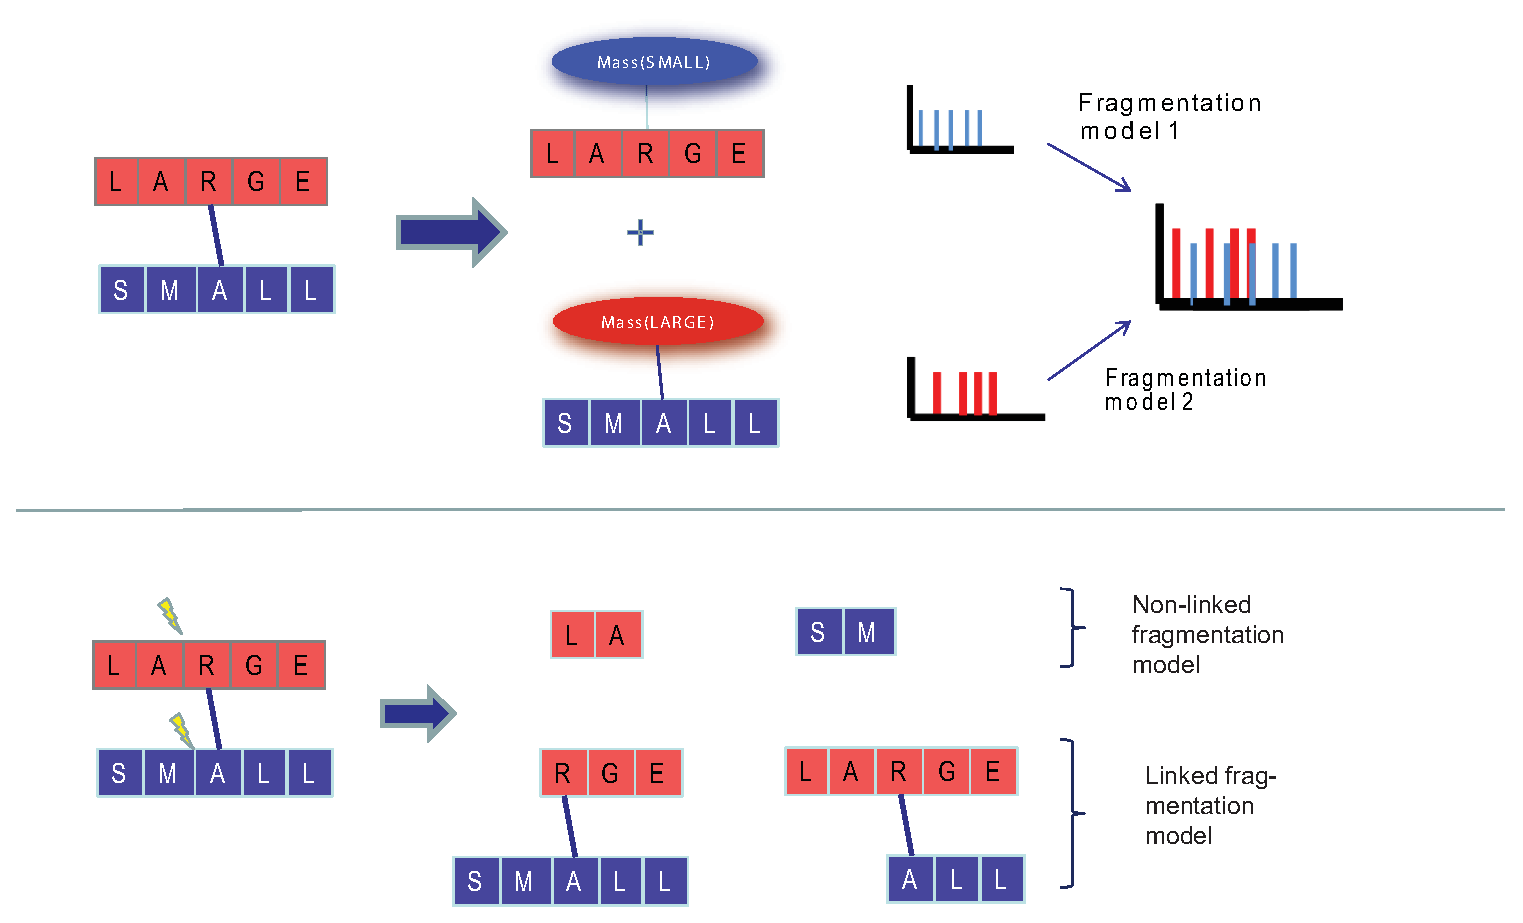
\includegraphics[height=80mm, width=160mm]{figures/Disulfide_fragment_model.eps}
		\caption{\footnotesize{\bf Linked peptides fragmentation model.} { {\bf Top panel:} to account for fragment ions from both linked peptides, we model a linked peptide as a mixture of two peptides where each carries a modification with mass equal to the mass of the other peptide plus the mass of the linker (which can possibly be negative, as is the case for disulfide bonds). To generate a theoretical spectrum for a linked peptide pair, our probabilistic model separately generates a theoretical spectrum for each peptide in the pair and then combines them into the theoretical spectrum for the linked peptide pair. This allows for separate modeling of each linked peptide and can thus capture statistical differences in fragmentation patterns (e.g., when one peptide is long and the other is short). {\bf Bottom panel}: to better capture the specific fragmentation properties of linked peptides, our model separates fragment ions from linked peptides into two categories: linked-fragments and non-linked fragments. Linked fragments are peptide fragments that are covalently linked to a second peptide.  While the fragmentation statistics for non-linked fragments should share some similarity to those of linear, unlinked peptides, linked-fragments have substantially different fragmentation statistics than those of unlinked peptides. In particular we expect higher-charge fragments to be more prominent because linked-fragments carry a second peptide and thus may have an extra N-termini and C-termini tryptic residue to attract charges. Thus in our probabilistic models for linked peptides, all theoretical fragment ions are separated into linked and unlinked fragments, each with separately estimated ion fragmentation statistics.}}
\label{linkedmodel}
\end{figure}

Linked peptides can also arise from various experimental protocols designed to covalently hold proteins together. For example, chemical crosslinking has been shown to be a powerful tool to study protein-protein interactions and to help elucidate the structure of large protein complexes~\cite{Sinz06,stengel2012joining,herzog2012structural}. In such experiments, chemical crosslinkers are added to the samples so pairs of reactive amino acid residues that are spatially close become covalently linked to one another.  Subsequent detection of these linked residues can provide structural information about protein structure and interactions. When the linked residues are from the same protein (intra-protein crosslink), they provide distance constraints to deduce the possible conformation of the protein structure. On the other hand, when the linked residues come from different proteins (inter-protein crosslink) they provide direct evidence that two proteins are in physical contact with each other.

Despite the importance of linked peptides to help us understand the function, structure and interactions of proteins, computational tools to identify linked peptides are still in their infancy.  There are three major computational challenges in developing tools for identification of linked peptides.
%
First, the covalent linkage of two peptides changes the physicochemical properties of the peptides and thus generates new types of fragment ions which display substantially different fragmentation statistics than those captured by current models for linear, unlinked peptides.
%
Second, spectra from linked peptides contain a mixture of fragment ions from \emph{two} peptides, which is not easily handled by current tools since almost all of them make the assumption that each spectrum comes from a single peptide. The presence of two peptides in the same spectrum also creates a quadratic search space for peptide candidates, where the number of linked-peptide candidates is in the order of $10^{8}-10^{11}$. Efficient techniques are thus needed to efficiently search this vast search space.
%
Finally there is only a very limited number of reliably identified publicly available spectra to learn the fragmentation models for linked peptides, thus making the development of these tools quite difficult. This situation is not easily amended because without efficient computational tools to identify MS/MS spectra from linked peptides in the first place, it is almost impossible to construct a large annotated training dataset for linked peptides, a ``chicken-and-egg'' problem.  Below we outline how we aim to break this vicious cycle to expedite the development of identification tools for any type of linked peptides.

% Extended introduction

%*******************************************
\section{Innovation}
%*******************************************
We propose new probabilistic scoring models that capture the fragmentation characteristics of linked peptides.  A linked peptide spectrum is modeled as a spectrum from a pair of peptides in order to account for all the possible fragment ions from both peptides (Figure~\ref{linkedmodel}a) and the proposed models explicitly address the co-fragmentation of a pair of peptides to score a linked peptide match to an observed spectrum.  
%This framework also allow us to build separate scoring model for each of the linked peptides, accounting for their difference in fragmentation statistics. 
Our proposed models further separate fragment ions into linked and unlinked fragments to model the highly-charged fragment ions that are specific to linked peptides (Figure~\ref{linkedmodel}b).  With this new scoring function we derive a filtration strategy based on the concept of vector projection to filter the search space of all possible peptide pairs by several order of magnitude.  Finally in order to obtain a training dataset we utilize combinatorial peptide synthesis~\cite{houghten1991generation} to efficiently generate a large set of linked peptides and couple it with a search strategy that takes advantage of the special design of the peptide library to identify MS/MS spectra from these linked peptides.


%*******************************************
\section{Approach}
%*******************************************
\subsection{Aim 3: Universal tool for identification of linked peptides}

%\subsubsection*{UniLink}
%\begin{itemize}
%    \item Fragmentation model
%    \item Synthetic libraries for learning models
%    \item Results on crosslinked vs xQuest and SUMO
%\end{itemize}

\subsubsection{Generate training data using combinatorial peptide synthesis}

In order to obtain a large training dataset for linked peptides we designed and synthesized combinatorial peptide libraries (Figure~\ref{librarybuild}). Peptide libraries are designed with the goal of maximizing sequence diversity while also representing a realistic model of endogenous linked peptides. While this low-cost approach necessarily limits the diversity of peptide sequences, the resulting peptide fragmentation models allow us to derive initial models be used to obtain a set of identifications for endogenous linked peptides from which the models can then be iteratively retrained. Conversely, combinatorial libraries can also be used to derive fragmentation models for types of peptides that are difficult to identify from cell lysates \-- for example, linked peptides connecting long peptides to short peptides (since MS/MS fragmentation tends to be dominated by ions from the long peptide and complicates the identification of the short peptide).

MS/MS spectra from linked peptide libraries were first analyzed using existing tools to define the initial training dataset. These were then used to learn the parameters of the peptide fragmentation models and to derive a scoring model tailored to linked peptides. Finally using this improved scoring model we searched once again through all MS/MS spectra from the peptide library to identify a final list of linked-peptides spectra. This approach was applied to generate reference MS/MS data for two types of linked peptides: SUMOylated peptides (i.e., ``Y-shaped'' linked peptides) and disulfide-bridged peptides (i.e., ``H-shaped'' linked peptides). The overall workflow of generating training data for SUMOylated peptides is illustrated in Figure~\ref{librarybuild}. Using this approach we have successfully generated training data from SUMOylated peptides in library I and II and demonstrated that our new method improves the identification of SUMOylated peptides in biological samples (detailed below). Current SUMO fragmentation models can be further improved by designing and using peptide libraries with a more diverse representation of possible endogenous SUMOylated peptides.
% Further improvement to the SUMO models can be done by designing peptide library that has more realistic representation of endogenous SUMOylated.  One such example is shown in peptide library III where we plan to incorporate the known consensus motif for SUMOylation into the sequence pattern.  
During our analysis of the training data we observed that peptide libraries I and II have different fragmentation statistics due to the different conjugating sites of the SUMO tag. Thus, to make our modeld more comprehensive we also plan to synthesize another library with the SUMO attachment site closer to the C-term of the substrate peptides.

\begin{figure}[h!]
	\centering
		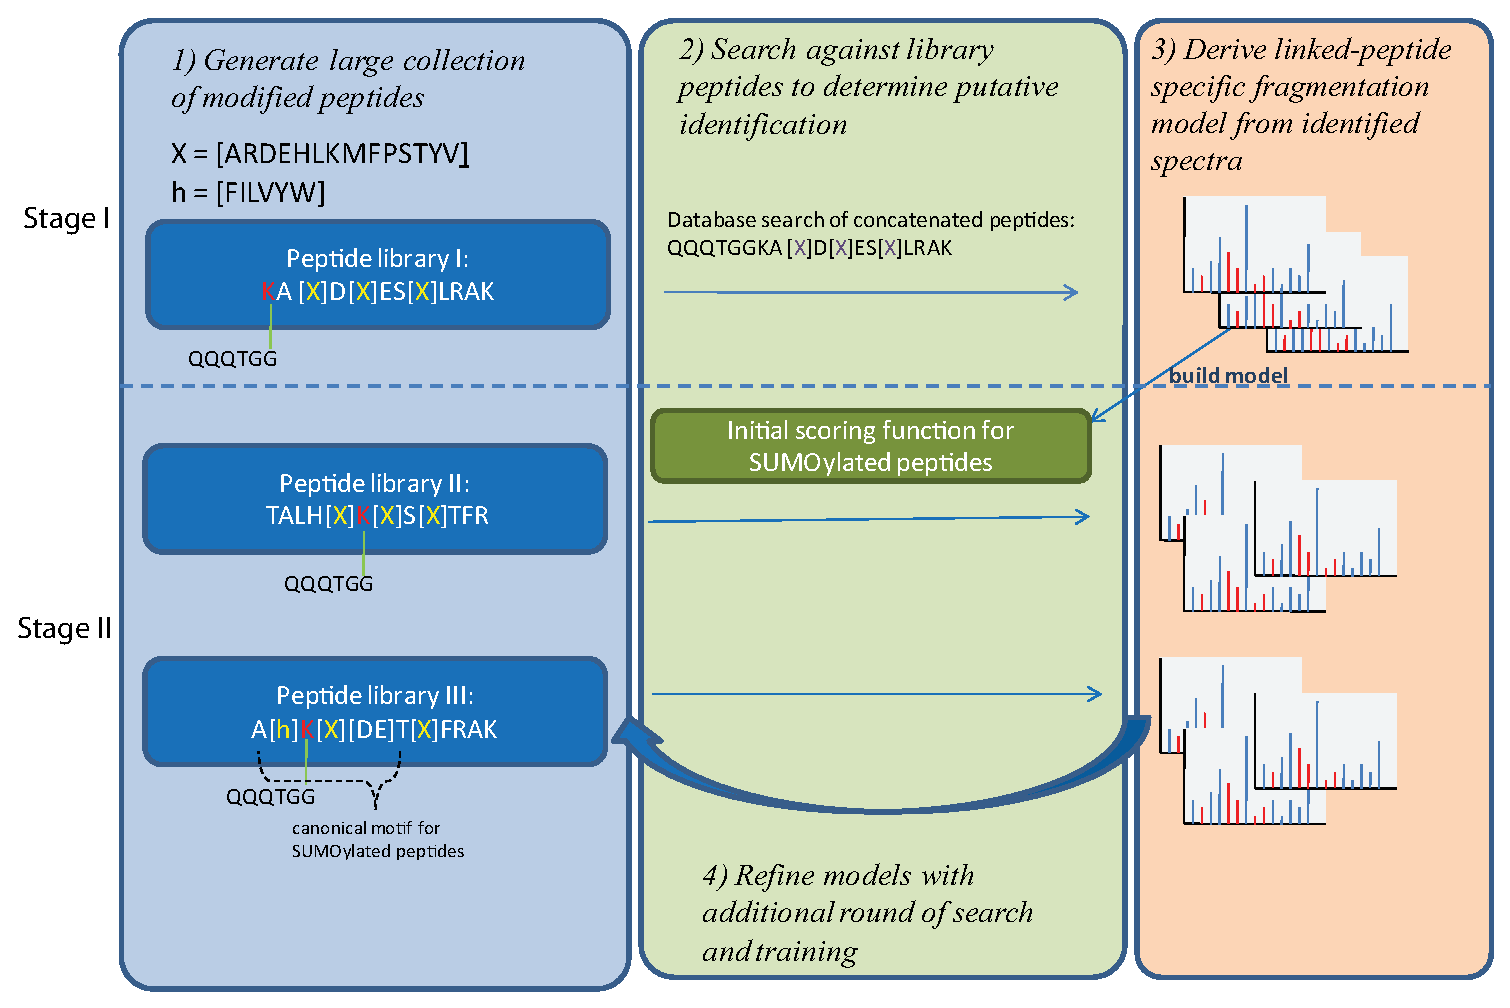
\includegraphics[height=100mm, width=150mm]{figures/Sumo_library_construction}
		\caption{{\bf Generating training data for linked peptides using combinatorial synthetic peptide libraries.} {\footnotesize In order to generate a large training dataset for SUMOylated peptides we designed and synthesized three combinatorial peptide libraries, each with a SUMO tag (QQQTGG) attached via a Lysine residue at a different position along the library peptide {\em (step 1)}. The sequence pattern for each library is shown on the left.  The symbols $X$ and $h$ stand for variable positions where multiple amino acid residues are possible, as indicated in the upper left corner.  MS/MS spectra from these peptide libraries are identified using a two-stage search strategy.  For library $I$, the SUMO tag is attached to the library peptide at the first residue.  Conceptually this is nearly equivalent to the substrate peptides having a prefix extension of QQQTGG. But since the SUMO tag is attached to the N-term Lysine and not to the N-term itself, the peptide fragmentation patterns are already expected to represent those of endogenous linked peptides with a similar structure of near-N-term linkage. We can identify MS/MS spectra from library $I$ by searching a custom database where the sequence QQQTGG is concatenated to N-term of every possible peptide sequence in library $I$, thus allowing us to identify an initial set of MS/MS spectra from SUMOylated peptides {\em (step 2)}. From this set we built a database search method specifically for SUMOylated peptides {\em (step 3)} and used it to identify MS/MS spectra from peptide libraries $II$ and $III$ which are more realistic representations of SUMOylated peptides seen in biological samples (e.g., library $III$ encodes the canonical SUMO motif). Identified spectra from libraries $II$ and $III$ were then incorporated into the training set to build a more general scoring model for SUMOylated peptides {\em (step 4)}. Finally, we use the improved method to search the spectra from all three libraries once again to identify a final set of MS/MS spectra from SUMOylated peptides.}}
\label{librarybuild}
\end{figure}

A similar approach to that illustrated in Figure~\ref{librarybuild} was used to generate training data for disulfide-bridged peptides, except that in the initial round of searching (step 2 in Figure~\ref{librarybuild}) we used the scoring function learned from SUMOylated peptides. The sequence patterns used for the disulfide peptide libraries were: $I)$ \mbox{K[AW][DE]F[VSHY]A[DY]SCVA[KR]}, $II)$ \mbox{[TW]A[LE]H[FV]SCVT[PSGY]F[KR]} and
$III)$ \mbox{[WA]VK[FL]C[DE]T[VSGY]FA[KR]}. In theory this approach can be used to generate data for cross-linked peptides with any cross-linkers. However, during our initial testing, we found that the yield of cross-linked peptides from peptides libraries is quite low (only a few percentage of peptides form dimers), possibly due to the fact that peptides in solution are relative far apart and the cross-linkers got hydrolyzed before they can react with the peptides.  We propose to address this issue by generating cross-linked peptides using disulfide-bridged peptides as a scaffold. After peptides in the library form disulfide-bridges and thus become spatially close to each other, we will $i)$ add cross-linkers to the dimers and $ii)$ reduce the disulfide bonds to create cross-linked peptides. Using this procedure we expect to be able to efficiently generate training data for cross-linked peptides with any available crosslinkers.

% After synthesis the peptide libraries were put in condition to promote the formation of random disulfide-bridged dimers.

\subsubsection{Linked peptides statistical fragmentation models}

A match between a linked peptide pair and an observed MS/MS spectrum is modeled as a mixture of two peptides, with each peptide carrying a modification at the cross-linked residue with mass equal to the mass of the linker plus the mass of the other peptide (Figure~\ref{linkedmodel}). In regular database search for unlinked peptides, one evaluates how well a \emph{single} candidate peptide matches to a given MS/MS spectrum. For crosslinked peptides we evaluate how well a \emph{pair} of peptides matches to a given MS/MS spectrum.  The probabilistic scoring models used for linked peptides is similar to that described in UniQuest (see Aim 1).  We will extend this model to further describe the fragmentation of a pair of peptides and also the specific fragmentation of linked fragment ions. Similar to UniQuest, we aim to develop universal probabilistic models for linked peptides.

Briefly, an MS/MS spectrum is represented as a vector of $n$ bins, each representing a mass interval of width $\delta$ Da ($\delta$ depends on instrument resolution).  An experimental MS/MS spectrum is represented as a vector $S = s_{1}, s_{2}, ... s_{n}$ where $s_{i}$ represents the peak intensity rank (ranked from most to least intense) of the highest-intensity peak in each bin.  Similarly, a theoretical spectrum of a peptide $P = p_{1}, p_{2}, ... p_{n}$ is represented as a vector where $p_{i}$ indicates the ion-type of the fragment ion (e.g. b-ion or y-ion) with mass in that bin.  The model captures peptide fragmentation statistics by using a set of annotated MS/MS spectra to learn the probability that each type of ion generates an observed peak with a given rank: $Prob(s|p)$.  Similarly a noise $Prob(s|0)$ model can be learned using unmatched peaks in the spectrum (where the symbol $0$ represents noise). The scoring function for a Peptide Spectrum Match (PSM) is thus defined as likelihood ratio of the probability that the observed spectrum $S$ is generated from the candidate peptide $P$ versus the probability that the observed spectrum is generated from noise: $Score(S,P)=\sum{Score(s_{i}}, p_{i})=\sum{log(\frac{Prob(s_{i}|p_{i})}{Prob(s_{i}|0)})}$. Since linked peptides are represented as pairs of peptides, we can represent a linked peptide as two vectors $(P, Q)$. The vector $P = p_{1}, p_{2}, ... p_{n}$ contains all possible fragment ions from the first peptide while the vector $Q = q_{1}, q_{2}, ... q_{n}$ contains all possible fragments ions from the second peptide.  Without loss of generality, we define the first peptide to be the dominant peptide that accounts for more ion intensity in the observed MS/MS spectrum.  This way we can account for possible differences in fragmentation patterns between the first and second peptides.  The score that a spectrum $S$ is matched to a pair of peptides $(P,Q)$ is thus: $Score(S,(P,Q)) = \sum_i{\max(Score(s_{i}|p_{i}), Score(s_{i}|q_{i}))}$, where $\max$ is used to model the dependency between the two peptides. When theoretical fragment ions from both $P$, $Q$ match to the same observed spectrum peak, the model only uses the fragment ion with higher probability, thus avoiding using the same peak twice to support the identification of linked peptides. If not explicitly prevented, such double-counting will incorrectly bias unusually high scores towards pairs of peptide candidates sharing many of their theoretical fragment ions.

In order to further capture the fragmentation statistics of crosslinked peptides we further divide the set of fragment ion types into linked and non-linked fragments (Figure~\ref{linkedmodel}). Linked fragments are fragment ions that are covalently linked to a second peptide.  Thus for every ion type that is used to describe linear peptides we introduce its corresponding linked ion type in our probabilistic models.  For example in our current implementation, we considered the ion types:  $b, b(iso), b-H2O, b-NH3, y, y(iso), y-H20, y-NH3$ for linear peptides, where $b(iso)$ indicates the first $^{13}C$ isotopic peak of a b-ion. Then we add the ion types $b_{X}, b(iso)_{X}, b-H2O_{X}, b-NH3_{X}, y_{X}, y(iso)_{X}, y-H2O_{X}, y-NH3_{X}$ to represent the corresponding linked-fragment ions that can be generated from linked peptides. For each ion type we consider charge states from one to the precursor charge of the observed MS/MS spectrum.  With these new ion types, the fragmentation statistics specific to linked peptide fragments can be learned during training and different probability/weights are assigned to linked and non-linked fragment ions.  Of course, in the full implementation of UniLink (as in UniQuest) we will make no special assumption about the ion types presented \-- all the ion types will be learned from the training data.

\subsubsection{Efficient database search for linked peptides}

We propose a two-step search strategy to avoid the quadratic search space of all possible linked peptides.  Since we model linked peptides as a pair of modified peptides, each with a modification at the linking site, we argue that for a linked peptide pair generating the observed spectrum, each peptide should score reasonably well when matched to the spectrum alone. Thus in the first stage of our search we will match every peptide candidate against the query spectrum and sort them by their match score.  In the second stage only the top N scoring peptides are then paired with the remaining candidates to find the best-scoring linked peptide pairs.  More concretely, let $S$ be a query MS/MS spectrum with parent mass $M_{S}$, let $P$ be a peptide with parent mass $M_{P}$ and consider a protein database that contains $n$ peptides ${P_{1}, P_{2}, ...... P_{n}}$. A modified peptide $P^m+\Delta_{t}$ is  peptide $P$ with a mass-offset of $\Delta$~Da at the $t$-th amino acid residue. For each peptide $P_{i}$ in the database we consider all of its modified variants $P^m_{i}+\Delta_{t}$, where $\Delta$ is the mass difference between the mass of the observed spectrum and the mass of the candidate peptide:  $\Delta = M_{S} - M_{P_{i}}\ \  s.t. \Delta > 0$ and $t$ is all valid linking sites for the candidate peptide $P_{i}$. For example, in the case of disulfide-bridged peptides, all cysteine residue positions are considered. We score all of these modified candidate peptides against the query spectrum $S$ and sort all the peptide candidates according to their match score. In our training data, we found that in more than $96\%$ of cases one of the linked peptides ranked 50 or less when searching against an E.Coli database.  Thus, rather than considering all possible peptide pairs, we take each of the top 50 peptide candidates and pair it with the remaining candidates in the database (such that their combined masses match the precursor mass of the observed MS/MS spectrum) to find the best-scoring linked peptide pair in the database.

\subsubsection{Preliminary results}
In order to test UniLink's performance, we first evaluated the SUMO models on three different datasets. The first  dataset contain a set of synthetic SUMOylated peptides from the Human Myeloid cell leukemia protein (MCL1) spiked in a background of human cell lysate. The other two datasets are from published studies of endogenous SUMOylated peptides in Arabidopsis~\cite{miller2010humansumo} and Human~\cite{matic2010site}. As shown in Figure~\ref{linkedIds}a, UniLink is able to identify 82.8\%--325\% more SUMOylated peptides than InsPecT~\cite{tanner05} or Mascot~\cite{mascot99}.  Since we do not currently have datasets that contains disulfide-bridged peptides from biological samples, we tested our disulfide-bridged models on two datasets from crosslinking studies on S.~Pombe and on Rabbit proteasome using the crosslinker DSS~\cite{leitner2012expanding}.  Although it is suboptimal to not have DSS-specific fragmentation models, we assess the performance of UniLink under the assumption that cross-linked peptides have fragmentation characteristics similar to disulfide-bridged peptides.  As shown in Figure~\ref{linkedIds}, UniLink is able to identify significantly more cross-linked peptides than the current state-of-the-art approach xQuest~\cite{rinner2008}.

\begin{figure}[h!]
	\centering
		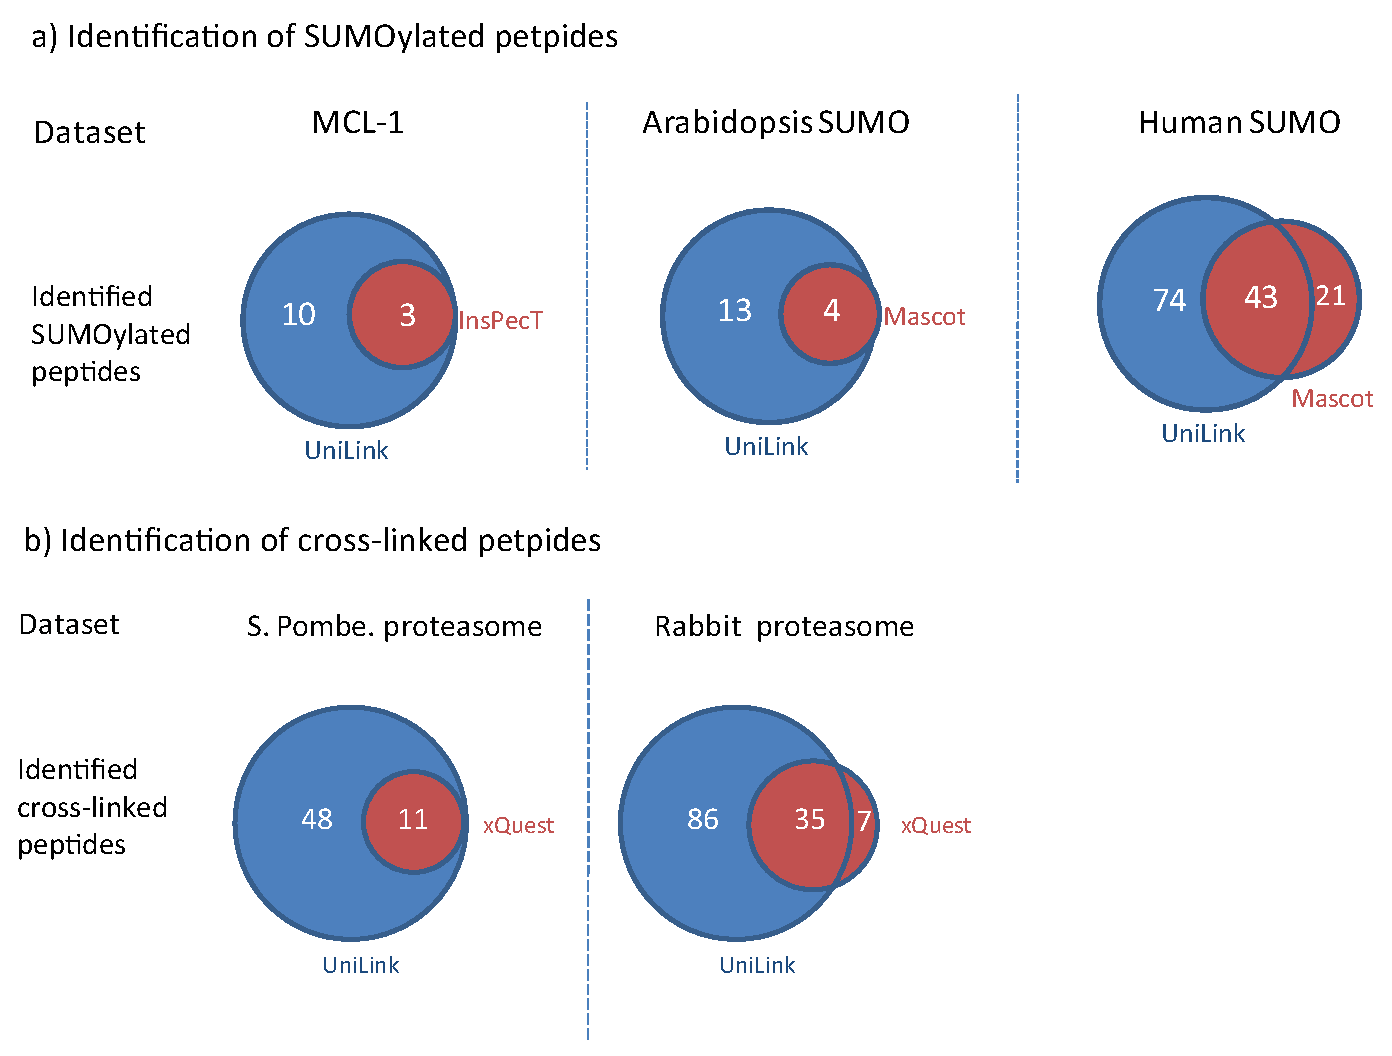
\includegraphics[height=100mm, width=150mm]{figures/linkedIDs_results.eps}
		\caption{{\bf UniLink identification of linked peptides.} {\footnotesize {\bf a)} The performance of UniLink for identification of SUMOylated peptides was tested in three datasets.  The MCL1 dataset contains 20 synthetic SUMOylated peptides from MCL1 spiked in a background of human cell lysate.  The Arabidopsis~\cite{miller2010humansumo} and Human SUMO~\cite{matic2010site} datasets were reanalyzed from two previous proteomics studies where identification of SUMOylated proteins and peptides have been reported. As shown, UniLink is able to improve the identification of SUMOylated peptides by 82.8\%--325\%. {\bf b)} UniLink was tested on cross-linked peptides using two datasets from crosslinking studies on protein complexes: the S.Pombe 26S proteasome and the Rabbit 20S proteasome~\cite{leitner2012expanding} were crosslinked with the commercial crosslinker DSS and then subsequetly analyzed by MS/MS. As shown UniLink is able to identify at least 288\% more crosslinked peptides than the current state-of-the-art tool xQuest.}}
\label{linkedIds}
\end{figure}

\subsubsection{Improving UniLink search efficiency and scoring models}

%With a new scoring function that are able to capture the specific fragmentation of linked peptides, we've demonstrated that it is able to improve our sensitivity of identifying linked peptides.  Conceptually, with our new scoring several techniques that has been used to improve the identification of single-peptide spectrum can seemlessly extended for the identification of linked peptides.  One such technique is tag-based filtering.  Note that although in 
UniLink avoids searching all possible linked peptide pairs by using the two-stage search strategy described above.  However, since the first stage is essentially a blind modification search, UniLink needs to consider almost every peptide candidate in the database.  This search space is considerably larger than regular database search of single-peptide spectra where one can filter the peptide candidates using parent mass filters. As previously shown by CCMS, tag-based filtering can be used to substantially speed up regular~\cite{tanner05} and blind~\cite{na2012} modification search of regular unlinked peptides. A similar strategy can be used for linked peptides by $i)$ using an appropriate peptide fragmentation model and $ii)$ extending sequence tagging algorithms to process spectra of linked peptides (e.g., sequence tags may need to span multiple fragment ion charge states).
%except that the scoring function that evaluate how likely a sequence-tag can be generated from the observed spectrum needed to updated to our new scoring function that properly captuer the fragmentation pattern of linked peptides.

The generating function approach (MSGF~\cite{kim2008}) introduced by CCMS to compute the statistical significance for PSMs was shown to greatly improve identification of unlinked peptides.  We propose to extend this concept for linked peptides by introducing two modifications to the original MSGF approach. First, an MSGF-compatible scoring function for linked peptides is required. Since the MSGF approach is applicable with any additive scoring function, we expect that the probabilistic models described above will be easily integrated into the MSGF framework.  Second, we need to extend the MSGF approach to the two-peptide case since a linked peptide spectrum is modeled as spectrum of two peptides with PTMs. This extension is loosely related to the MSGF extension proposed in TRD~7 for identification of multiplexed spectra from co-fragmentation of multiple co-eluting precursor peptides.

%\begin{itemize}
%    \item Tag-based filters
%    \item Link-GF as extension of MixGF
%    \item Blind-linker searches
%\end{itemize}

%**************************************************************************************
% ------------------------------------------------------------------------------------
\section{Summary}
% ------------------------------------------------------------------------------------
%**************************************************************************************

% Essentially summary of Discussion from papers + a paragraph on the new things proposed here.

%**************************************************************************************
% ------------------------------------------------------------------------------------
\section{Driving Biomedical Projects (DBPs)}
% ------------------------------------------------------------------------------------
%**************************************************************************************

% For all 3 aims

%\bibliographystyle{plain}
\bibliographystyle{unsrt}
\bibliography{../bibtex/msms_sort_unique}
\end{document}
